\section{Preliminares}

\begin{figure*}[!t]
  \centering
  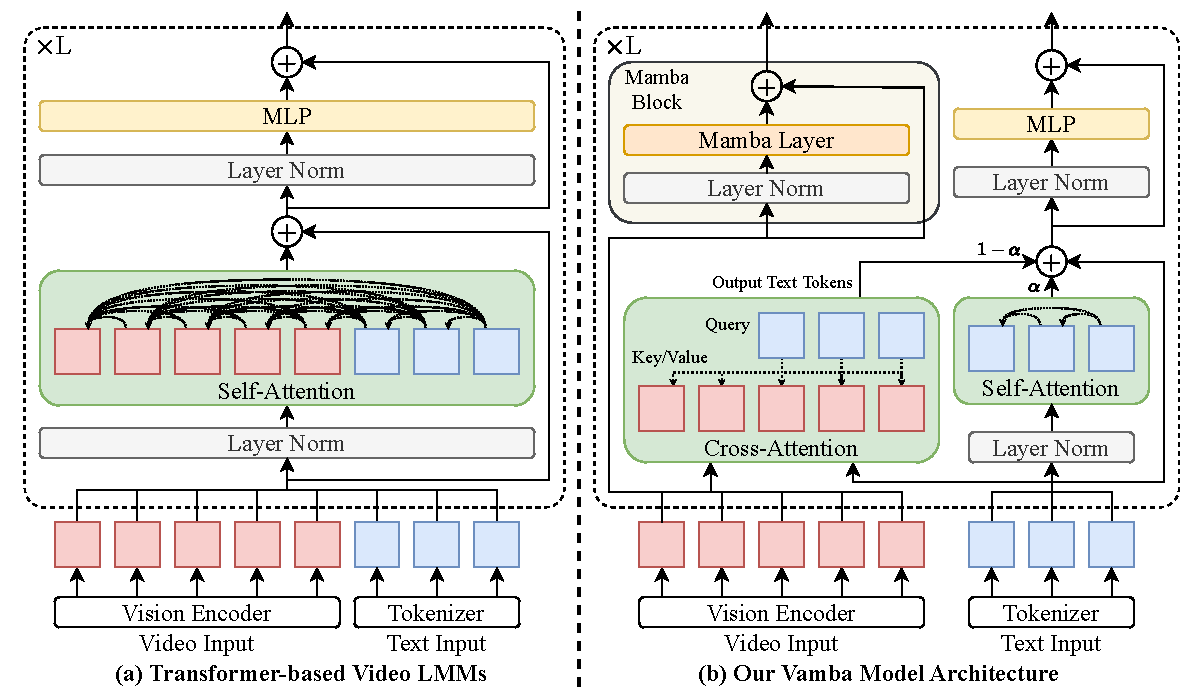
\includegraphics[width=0.9\textwidth]{figures/fig_attention.pdf}
  \vspace{-1em}
  \caption{Vista general de la arquitectura de nuestro modelo \model. En comparación con los LMMs basados en Transformer (izquierda), reemplazamos las costosas operaciones de causal self-attention por capas cross-attention y bloques Mamba más eficientes para lograr una mejor eficiencia.}
  \label{fig:main_attention}
  \vspace{-1em}
\end{figure*}

\subsection{State Space Models y Mamba}
Los state space models (SSMs) son sistemas lineales invariantes en el tiempo para modelar señales continuas. Un SSM continuo puede expresarse mediante ecuaciones diferenciales ordinarias (ODEs):
\begin{align*}
    h^\prime(t) = \mathbf{A}h(t) + \mathbf{B}x(t), \quad y(t) = \mathbf{C}h(t),
\end{align*}
Aquí, $x(t)\in \mathbb{R}$ es la señal de entrada, $h(t) \in \mathbb{R}^N$ es el hidden state de dimensión $N$ y $y(t) \in \mathbb{R}$ es la señal de salida. $\mathbf{A}\in \mathbb{R}^{N\times N}$ es la matriz de transición de estado y $\mathbf{B} \in \mathbb{R}^{N \times 1}, \mathbf{C}\in \mathbb{R}^{1\times N}$ son matrices de proyección.

Mamba \cite{gu2023mamba}, y su predecesor S4 \cite{gu2021efficiently}, son SSMs discretizados para discrete sequence modelling. La discretización del SSM se realiza mediante la técnica zero-order hold (ZOH):
\begin{align*}
\begin{split}
    \overline{\mathbf{A}} = \mathrm{exp}(\Delta\mathbf{A}), \quad \overline{\mathbf{B}} = (\Delta \mathbf{A})^{-1}(\mathrm{exp}(\Delta\mathbf{A}) - \mathbf{I})\cdot \Delta \mathbf{B},
\end{split}
\end{align*}
donde $\overline{\mathbf{A}},\overline{\mathbf{B}}$ son variables de estado discretizadas y $\Delta$ es el tamaño de paso. El SSM discretizado puede reescribirse como:
\begin{align*}
    h_t = \overline{\mathbf{A}}h_{t-1} + \overline{\mathbf{B}}x_t, \quad y_t = \mathbf{C}h_t.
\end{align*}

Mamba propone el algoritmo selective scan que determina dinámicamente $\mathbf{B}, \mathbf{C}, \Delta$ en función de las entradas de la secuencia. Siguiendo a S4, la matriz $\mathbf{A}$ se inicializa como la matriz HiPPO diagonalizada \cite{gu2020hippo}. Se ha demostrado que estas decisiones de diseño son eficientes y efectivas para modelar secuencias extremadamente largas. Mamba-2 \cite{dao2024transformers} simplifica aún más la formulación de $\mathbf{A}$ a una estructura escalar por identidad. Mamba-2 soporta multi-head SSM y permite una dimensión de estado $N$ mucho mayor que Mamba, al tiempo que es más rápido durante el entrenamiento.


\subsection{LMMs basados en Transformer}
\label{sec:autoregressive_lmm}
Estudiamos cómo se actualizan los tokens de texto y video en Transformers. Como se muestra en la Figura~\ref{fig:main_attention}, asumimos un caso estándar en el que los video tokens se colocan antes de los tokens de texto e ignoramos los chat template tokens por simplicidad. En cada capa decoder del LMM, los tokens de video y texto se actualizan como sigue:
\begin{itemize}
    \item Todos los video tokens se actualizan mediante una capa de input layer normalization (LN), una capa self-attention, una capa post LN y una capa MLP final. También hay conexiones residuales para las capas self-attention y MLP. El $i^{\mathrm{th}}$ video token $v_i$ calcula self-attention a partir de los primeros $i$ video tokens:
    \begin{equation}
    \label{equ:causal_self_attention_video}
        o_{v_i}=(\sigma(\frac{q_{v_i} \mathbf{K}_{[v_1:v_i]}^\top}{\sqrt{d}})\mathbf{V}_{[v_1:v_i]})\mathbf{W}_{o},
    \end{equation}
    donde $\sigma(\cdot)$ denota la operación softmax, $q_{v_i}$ es el query vector de $v_i$ y $\mathbf{K}_{[v_1:v_i]}$, $\mathbf{V}_{[v_1:v_i]}$ son las matrices key y value de los primeros $i$ video tokens. $d$ denota la dimensión de los query y key vectors y $\mathbf{W}_{o}$ es la matriz de proyección de salida. $o_{v_i}$ representa la salida final del token $v_i$.
    \item Los tokens de texto comparten una ruta de actualización similar a la de los video tokens. Las actualizaciones self-attention son ligeramente distintas: para el $j^{\mathrm{th}}$ token de texto $t_j$, calcula self-attention a partir de todos los video tokens y de los primeros $j$ tokens de texto:
    \begin{equation}
    \label{equ:causal_self_attention_text}
        o_{t_j}=(\sigma(\frac{q_{t_j} [\mathbf{K}_v,\mathbf{K}_{[t_1:t_j]}]^\top}{\sqrt{d}})[\mathbf{V}_v,\mathbf{V}_{[t_1:t_j]}])\mathbf{W}_{o},
    \end{equation}
    donde $[\mathbf{K}_v,\mathbf{K}_{[t_1:t_j]}]$ y $[\mathbf{V}_v,\mathbf{V}_{[t_1:t_j]}]$ son las matrices key y value de la combinación de todos los video tokens y los tokens de texto hasta $t_j$.
\end{itemize}

La principal sobrecarga computacional en los LMMs basados en Transformer proviene de la \textbf{complejidad cuadrática de la self-attention sobre los video tokens}. Para superar este problema, diseñamos una arquitectura híbrida Mamba Transformer para procesar de forma distinta los tokens de texto y video. Los detalles de nuestra arquitectura de modelo se presentan en las secciones siguientes.
